% !TeX root = ../main.tex
\chapter{Unidad 3: Fundamentos de la mecánica ondulatoria}

\section*{Objetivo pedagógico}
\noindent\textbf{Objetivo.} Comprender la diferencia entre movimiento oscilatorio y ondulatorio, describir el movimiento armónico simple (MAS) y relacionar sus parámetros (frecuencia, período, amplitud, fase y longitud de onda) con la propagación del sonido y su aplicación en fonoaudiología, como en las audiometrías. Se incluyen ejemplos clínicos, actividades prácticas, recursos multimedia y ejercicios de autoevaluación pensados para estudiantes con poca formación matemática.

\noindent\textbf{Pregunta inicial.} ¿Por qué un tono grave suena diferente a uno agudo? ¿Cómo se relaciona el movimiento de un parlante con el sonido que escuchamos? ¡Esta unidad te ayudará a entender cómo las ondas sonoras llevan la información auditiva!

\section{Movimiento oscilatorio versus movimiento ondulatorio}

\subsection{Movimiento oscilatorio}
El movimiento oscilatorio es el vaivén repetitivo de una partícula alrededor de un punto fijo, como un columpio que sube y baja. En acústica, las partículas de aire o el tímpano vibran de esta manera cuando una onda sonora las alcanza.

\begin{quote}
    \textbf{Ejemplo clínico.} Durante una audiometría, el tímpano oscila al recibir un tono puro, como un resorte que vibra con cada sonido.
\end{quote}

\subsection{Movimiento ondulatorio}
El movimiento ondulatorio ocurre cuando una perturbación (como el sonido) viaja a través de un medio, llevando energía sin mover la materia permanentemente. Imagina las olas en el mar: el agua sube y baja, pero la onda avanza hacia la playa.

\begin{quote}
    \textbf{Ejemplo práctico.} Cuando hablas, las vibraciones de tus cuerdas vocales crean ondas sonoras que viajan por el aire hasta el oído de quien escucha, mientras las moléculas de aire solo oscilan en su lugar.
\end{quote}


\textbf{Actividad práctica.} Toca una cuerda de guitarra o usa un diapasón (o mira un video en YouTube). Observa cómo la cuerda oscila en su lugar, pero el sonido viaja hasta tu oído. Esto muestra la diferencia entre oscilación y propagación.

\section{Movimiento armónico simple (MAS)}

El movimiento armónico simple (MAS) es un tipo de oscilación regular, como el movimiento de un péndulo. En acústica, describe cómo vibran las partículas de aire o el cono de un parlante para crear un tono puro.

Una onda sonora simple se representa como:
\[
x(t) = A \cos(2\pi f t + \varphi),
\]
donde:
\begin{itemize}
    \item \textbf{Amplitud ($A$):} La ``altura'' de la onda, que determina el nivel (en metros o pascales).
    \item \textbf{Frecuencia ($f$):} Cuántos ciclos por segundo (en hertz, Hz). Define la altura del sonido (grave o agudo).
    \item \textbf{Período ($T$):} Tiempo de un ciclo ($T = 1/f$, en segundos).
    \item \textbf{Fase ($\varphi$):} Punto de inicio de la onda (en radianes).
\end{itemize}

\begin{quote}
    \textbf{Ejemplo clínico.} En una audiometría, un tono de 1000 Hz ($T = 1/1000 = 0.001$ s) hace vibrar el tímpano con una amplitud pequeña, que el oído percibe como un sonido de intensidad moderada.
\end{quote}

\begin{figure}[h]
    \centering
    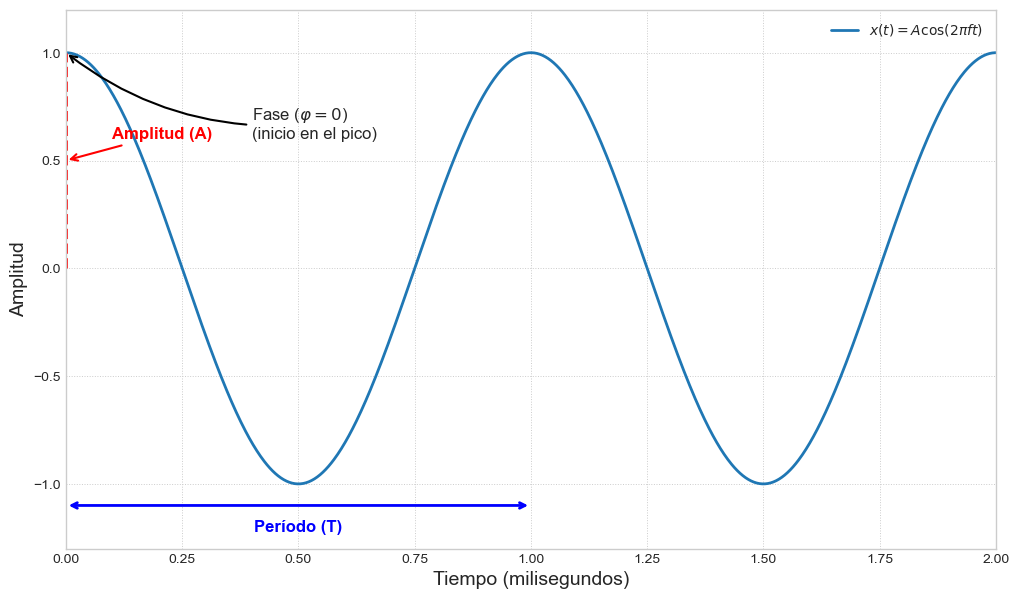
\includegraphics[width=1.0\textwidth]{figures/tono_1000.png}
    \caption{Onda sinusoidal de $f = 1000 Hz$, $A = 1$, $\phi = 0$ y $T=1, ms$.}
    \label{tono_1000}
\end{figure}


\subsection{Velocidad del movimiento}
La velocidad máxima de una partícula en MAS es:
\[
v_{\max} = 2\pi f A \quad \Biggl[\frac{m}{s}\Biggr].
\]
Por ejemplo, un parlante que vibra a 1000 Hz con una amplitud de 0.3 mm tiene una velocidad máxima de:
\[
v_{\max} = 2\pi \cdot 1000 \cdot 0.0003 \approx 1.9~\text{m/s}.
\]
Esto muestra cómo un movimiento pequeño produce un sonido audible.

\textbf{Actividad práctica.} Usa una app como Tone Generator (gratis en línea) para escuchar tonos de 250 Hz y 1000 Hz. Nota cómo el tono más agudo (1000 Hz) tiene una frecuencia mayor, lo que significa que las partículas vibran más rápido.

\section{Tono puro y su relevancia clínica}

Un \textbf{tono puro} es un sonido con una sola frecuencia, como el pitido de un audiómetro. En fonoaudiología, los tonos puros son esenciales para evaluar la audición en diferentes frecuencias (125 Hz a 8000 Hz).

\subsection{Relación longitud de onda–frecuencia}
La longitud de onda ($\lambda$) es la distancia que recorre una onda en un ciclo:
\[
\lambda = \frac{c}{f} \quad [m],
\]
donde $c$ es la velocidad del sonido (343 m/s en aire a 20°C, 1500 m/s en agua). Por ejemplo, un tono de 1000 Hz tiene:
\[
\lambda = \frac{343}{1000} \approx 0.34~\text{m} \text{ (en aire)}.
\]

\begin{table}[h]
    \centering
    \small
    \begin{tabular}{|c|c|c|c|}
        \hline
        \textbf{Frecuencia ($f$ [Hz])} & \textbf{Período ($T$ [ms])} & \textbf{$\lambda$ del aire [m]} & \textbf{$\lambda$ del agua [m]} \\
        \hline
        125 & 8.0 & 2.74 & 12.0 \\
        1000 & 1.0 & 0.343 & 1.50 \\
        4000 & 0.25 & 0.086 & 0.375 \\
        \hline
    \end{tabular}
    \caption{Período y longitud de onda de tonos puros usados en audiometrías.}
\end{table}

\begin{quote}
    \textbf{Ejemplo clínico.} En una audiometría, un tono de 4000 Hz (longitud de onda corta) prueba la audición de frecuencias agudas, comunes en el habla (como las consonantes ``s'' o ``f'').
\end{quote}

\begin{figure}[h]
    \centering
    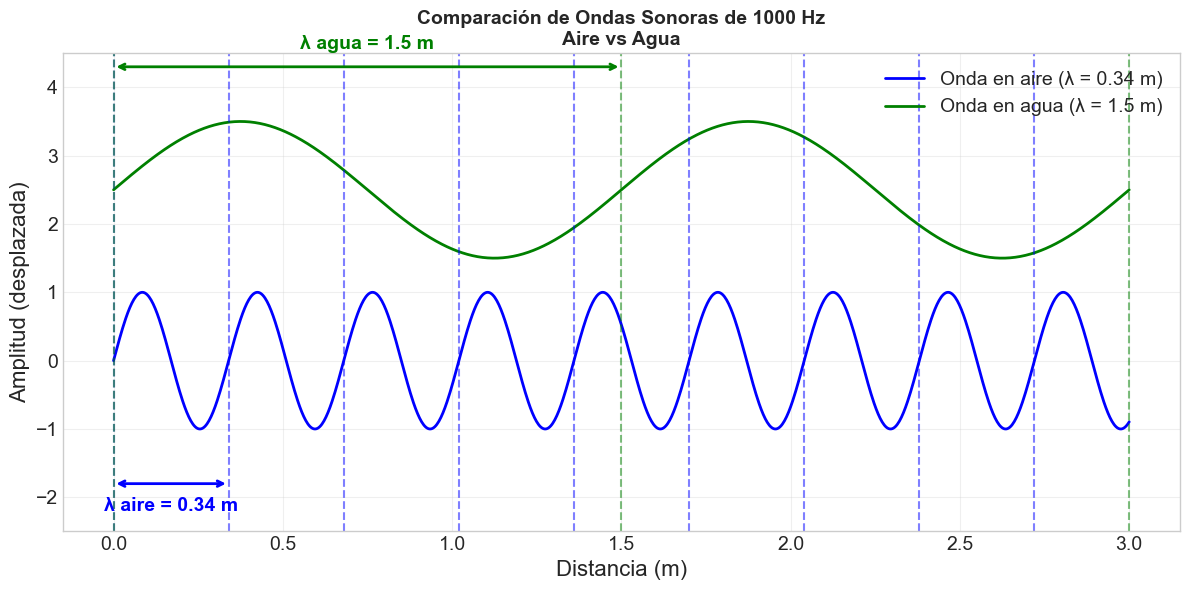
\includegraphics[width=1.0\textwidth]{figures/ondas_aire_agua.png}
    \caption{Logitud de onda de un tono de 1000 Hz en aire vs en agua.}
    \label{fig:ondas-aire-agua}
\end{figure}


\section{Fase y superposición}

La fase ($\varphi$) determina en qué punto comienza una onda. Cuando dos ondas de la misma frecuencia se combinan, su fase relativa puede sumarlas (interferencia constructiva, $\Delta\varphi = 0$) o restarlas (interferencia destructiva, $\Delta\varphi = \pi$).

\begin{quote}
    \textbf{Ejemplo clínico.} En audífonos con cancelación activa de ruido (ANC), se genera una onda con fase opuesta al ruido ambiental, reduciendo lo que escucha el usuario. Esto mejora la claridad de la voz en entornos ruidosos.
\end{quote}

\begin{figure}[h]
    \centering
    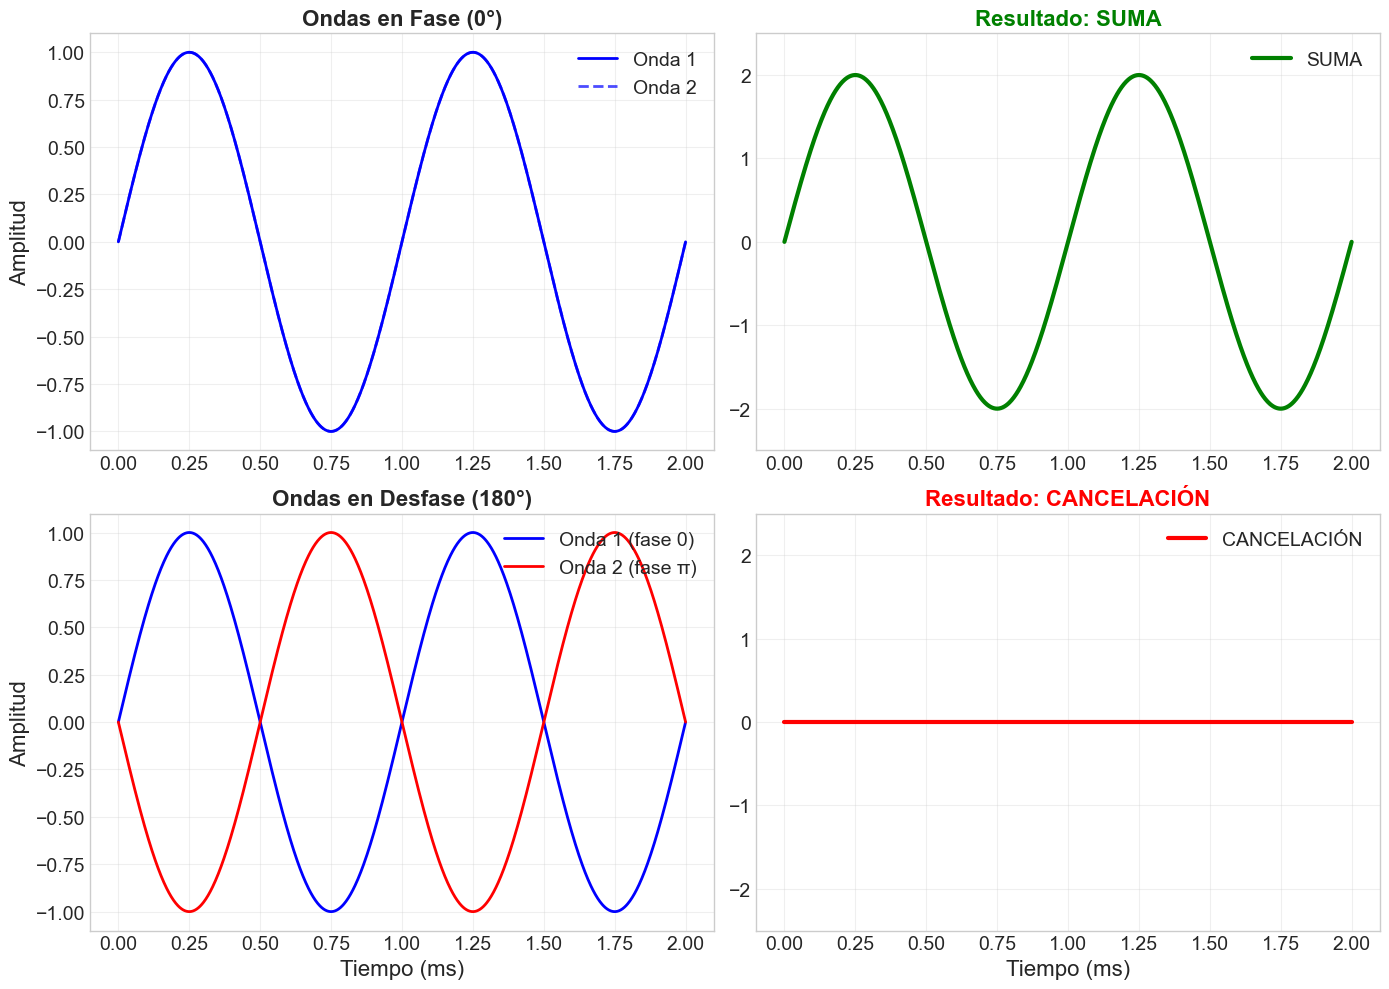
\includegraphics[width=1.0\textwidth]{figures/suma_ondas.png}
    \caption{Interferencia constructiva vs destructiva de una onda sinusoidal.}
    \label{fig:suma-ondas}
\end{figure}


\textbf{Actividad práctica.} Escucha un video de YouTube sobre cancelación de ruido (busca ``active noise cancellation'') y observa cómo los audífonos ANC reducen el ruido de fondo. Intenta identificar el principio de interferencia destructiva.

\section{Recursos recomendados}
\begin{itemize}
    \item Video: \href{https://www.youtube.com/watch?v=gZ_KnZHCn4M&ab_channel=ProfessorDaveExplains}{``Simple Harmonic Motion: Hooke's Law''}
    \item App: Tone Generator (gratis en línea). Genera tonos puros para experimentar con frecuencias.
    \item App: Audacity (gratis). Visualiza la forma de onda de tu voz o tonos puros.
    \item Libro: B. P. Kinsler \emph{et al.}, \emph{Fundamentals of Acoustics}, capítulos 4–5.
    \item Libro: L. L. Beranek, \emph{Acoustics}, sección 2.
\end{itemize}

\section{Ejemplos prácticos}

\subsection{Ejemplo 1: Cálculo de período y longitud de onda}
Para un tono de 2000 Hz en aire:
\[
T = \frac{1}{2000} = 0.5~\text{ms}, \quad \lambda = \frac{343}{2000} \approx 0.172~\text{m}.
\]
En agua:
\[
\lambda = \frac{1500}{2000} = 0.75~\text{m}.
\]
Esto muestra que las ondas son más largas en agua, afectando cómo se perciben los sonidos.

\subsection{Ejemplo 2: Velocidad de una partícula}
Un parlante vibra a 500 Hz con amplitud de 0.5 mm. La velocidad máxima es:
\[
v_{\max} = 2\pi \cdot 500 \cdot 0.0005 \approx 1.57~\text{m/s}.
\]
Esto ilustra cómo un movimiento pequeño produce un sonido audible.

\subsection{Ejemplo 3: Audiometría}
Un tono de 250 Hz ($T = 4$ ms, $\lambda = 1.37$ m en aire) se usa en una audiometría para evaluar frecuencias graves. Si el paciente no lo detecta, podría indicar pérdida auditiva en ese rango.

\section{Ejercicios de autoevaluación}
\begin{enumerate}
    \item Describe la ecuación de un MAS para un tono con amplitud de 2 mm, frecuencia de 250 Hz y fase inicial de $-\pi/4$ rad. (\emph{Solución}: $x(t) = 0.002 \cos(2\pi \cdot 250 t - \pi/4)$.)
    \item Calcula la longitud de onda en agua de un tono de 6000 Hz. (\emph{Solución}: $\lambda = 1500/6000 = 0.25$ m.)
    \item Escucha un tono de 500 Hz y otro de 2000 Hz en Tone Generator. ¿Cuál suena más agudo y por qué?
    \item Explica cómo la interferencia destructiva se usa en audífonos ANC para mejorar la audición en un entorno ruidoso.
\end{enumerate}

\section*{Glosario}
\begin{description}
    \item[\textbf{Amplitud ($A$):}] Máximo desplazamiento de una onda. Determina el volumen.
    \item[\textbf{Frecuencia ($f$):}] Número de ciclos por segundo (Hz). Define la altura del sonido.
    \item[\textbf{Período ($T$):}] Tiempo de un ciclo ($T = 1/f$). Mide la duración de una oscilación.
    \item[\textbf{Fase ($\varphi$):}] Punto de inicio de una onda, que afecta su combinación con otras.
    \item[\textbf{Longitud de onda ($\lambda$):}] Distancia entre dos puntos consecutivos en fase.
    \item[\textbf{Movimiento armónico simple (MAS):}] Oscilación regular, como la de un parlante.
    \item[\textbf{Tono puro:}] Sonido con una sola frecuencia, usado en audiometrías.
\end{description}

\section*{Resumen}
\begin{itemize}
    \item \textbf{Oscilación vs. ondulatorio:} Las partículas oscilan en su lugar, pero la onda transporta energía, como el sonido de la voz viajando al oído.
    \item \textbf{MAS:} Describe cómo vibran el tímpano o un parlante, con parámetros como amplitud (volumen) y frecuencia (altura).
    \item \textbf{Tono puro:} Esencial en audiometrías para evaluar la audición en frecuencias específicas.
    \item \textbf{Fase:} Afecta cómo se combinan las ondas, como en la cancelación de ruido.
\end{itemize}

\bigskip
\noindent\emph{Conclusión.} Comprender el movimiento oscilatorio, el movimiento armónico simple y los parámetros de las ondas (frecuencia, período, amplitud, fase, longitud de onda) es fundamental para analizar cómo se generan y propagan los sonidos. Estos conceptos te ayudarán a interpretar audiometrías, entender el diseño de audífonos y analizar fenómenos como la cancelación de ruido. En la próxima unidad, exploraremos las propiedades del sonido y su relación con la percepción auditiva.


%%%%%%%%%%%%%%%%%%%%%%%%%%%%%%%%%%%%%%%%%%%%%%%%%%%%%%%%%%%%%%%%%%%%%%%%%%%%%%%%%%%%%%%%%%%%%%%%%%
